%----------------------------------------------------------------------------------------
%	PACKAGES AND THEMES
%----------------------------------------------------------------------------------------
\documentclass[aspectratio=169,xcolor=dvipsnames]{beamer}
\usetheme{SimplePlusAIC}

\usepackage{hyperref}
\usepackage{graphicx} % Allows including images
\usepackage{booktabs} % Allows the use of \toprule, \midrule and  \bottomrule in tables
\usepackage{svg} %allows using svg figures
\usepackage{tikz}
\usepackage{makecell}
\newcommand*{\defeq}{\stackrel{\text{def}}{=}}

\makeatletter
\usepackage{tikz}
\usetikzlibrary{calc}
\newcommand*\circled[1]{\tikz[baseline=(char.base)]{
    \node[shape=circle, draw, inner sep=1pt, 
        minimum height={\f@size*1.6},] (char) {\vphantom{WAH1g}#1};}}
\makeatother

%Select the Epilogue font (requires luaLatex or XeLaTex compilers)
\usepackage{fontspec}
\setsansfont{Epilogue}[
    Path=./epilogueFont/,
    Scale=0.9,
    Extension = .ttf,
    UprightFont=*-Regular,
    BoldFont=*-Bold,
    ItalicFont=*-Italic,
    BoldItalicFont=*-BoldItalic
    ]

%----------------------------------------------------------------------------------------
%	TITLE PAGE
%----------------------------------------------------------------------------------------

\title[KFC]{Kinship Verification with Fair Contrastive Loss and Multi-Task Learning} % The short title appears at the bottom of every slide, the full title is only on the title page
%\subtitle{Subtitle}

\author[Barbosa, Warley .V]{Warley Vital Barbosa}
%\institute[FEE CTU]{Artificial Intelligence Center \newline Faculty of Electrical Engineering\newline Czech Technical University in Prague}
% Your institution as it will appear on the bottom of every slide, maybe shorthand to save space

\AtBeginSection[]
{
  \begin{frame}{Overview}
  \tableofcontents[
    currentsection,
    sectionstyle=show/hide,
    subsectionstyle=show/show/hide
  ]
  \end{frame}
}

\date{\today} % Date, can be changed to a custom date
%----------------------------------------------------------------------------------------
%	PRESENTATION SLIDES
%----------------------------------------------------------------------------------------

\begin{document}

\begin{frame}[plain]
    % Print the title page as the first slide
    \titlepage
\end{frame}

\begin{frame}{Overview}
    % Throughout your presentation, if you choose to use \section{} and \subsection{} commands, these will automatically be printed on this slide as an overview of your presentation
    \tableofcontents
\end{frame}

%------------------------------------------------
\section{Introduction}
%------------------------------------------------

\begin{frame}{Introduction}
    \begin{itemize} 
        \item Kinship Recognition (KR) is an important problem with applications like finding missing children and photo management. 
        \begin{itemize}
            \item \textbf{Facial KR} seeks to discover possible \textbf{kin relationships} between face images.
            \item Kinship Verification involves identifying the \textbf{degree of relatedness} between individuals based on their \textbf{unique facial features}.
        \end{itemize}
        \item Human faces contain not only \textbf{family information} but also \textbf{racial traits}.
        \item However, researchers \textbf{focus} more on accuracy performance than race and other biases.
        \begin{itemize}
            \item This has a \textbf{detrimental impact} on AI systems--healthcare, hiring algorithms, recidivism judgment, etc.
        \end{itemize}
    \end{itemize}
\end{frame}

%------------------------------------------------

\begin{frame}{Previous works on fairness in face recognition and face verification}
    \begin{itemize}
        %\item Fairness-aware loss function
        \item \cite{R22} exploits the interrelation between anchor and sample to design a \textbf{sensitive attribute removing} loss function.
        \item \cite{R42} uses \textbf{instance False Positive Rate} (FPR) in loss function to constrain bias.
        \item \cite{R39} implemented \textbf{post-processing data perturbation} without changing their parameters and structures that can \textbf{hide the information} of protected attributes.\
        \item \cite{R11} proposed to include \textbf{demographic-adaptive layers} that make the model generate face representations for every demographic group.
    \end{itemize}
\end{frame}

%------------------------------------------------

\begin{frame}{Proposal}
    \begin{itemize}
        \item \textbf{Objective}
        \begin{itemize}
            \item Improve \textbf{racial fairness} while achieving \textbf{higher accuracy} on kinship verification.
        \end{itemize}
        %\item \textbf{Siamese Networks} and Attention mechanisms are popular methods that focus on the most \textbf{critical regions} with unique facial features.
    \end{itemize}
\end{frame}

%------------------------------------------------

\begin{frame}{Proposal}
    \begin{itemize}
        \item \textbf{Problems}
        \begin{itemize}
            \item \textit{Fairness and small datasets} 
            \begin{itemize}
                \item \textbf{Combine and label} each individual's race in multiple kinship datasets -- KinRace
            \end{itemize}
            \item \textit{Boost accuracy and fairness simultaneously}
            \begin{itemize}
                \item A \textbf{fairness-aware loss function} in a multi-task learning framework.
            \end{itemize}
            \item \textit{Improve accuracy}
            \begin{itemize}
                \item \textbf{An attention module} that makes the model focus on the most representative facial regions for feature representation learning.
            \end{itemize}
            \item \textit{Improve fairness} 
            \begin{itemize}
                \item \textbf{Reverse the gradient of the race} classification branch to remove the racial information in the feature vector.
                \item A \textbf{fairness-aware contrastive loss} function that can mitigate pairwise bias and significantly decrease the standard deviation in four races.
            \end{itemize}
        \end{itemize}
    \end{itemize}
\end{frame}

%------------------------------------------------

\begin{frame}{Schematic}
    \begin{figure}
        \centering
        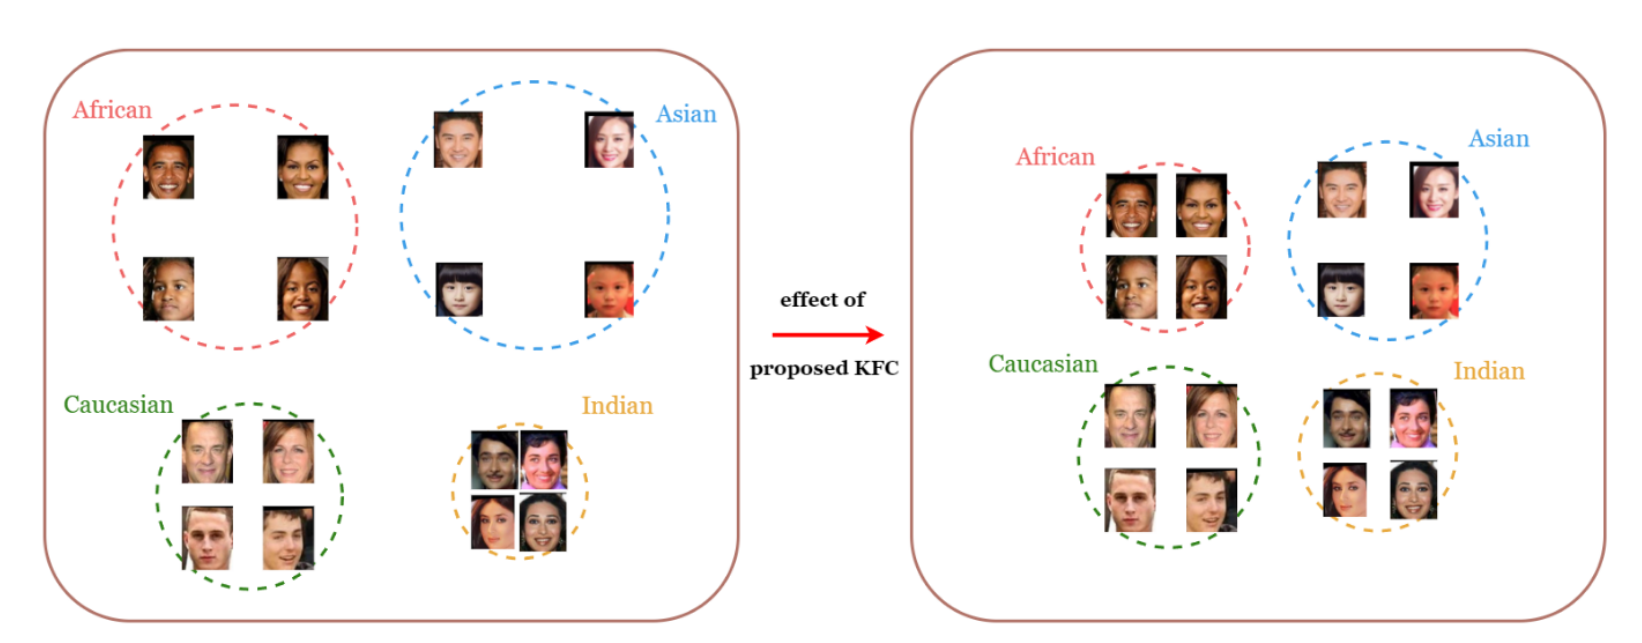
\includegraphics[width=0.75\textwidth]{imgs/1.png}
        \caption{From the authors. The schematic diagram for improving the fairness in kinship verification.}
        \label{fig:kfc-schematic}
    \end{figure}
    \begin{itemize}
        \item Their method effectively adjusts the \textbf{intra-class compactness} and \textbf{inter-class discrepancy} in the feature space.
        \item They mitigate bias by balancing four races' \textbf{intra-class and inter-class angles} and making them as \textbf{consistent} as possible.
    \end{itemize}
\end{frame}

%------------------------------------------------

\begin{frame}{Contributions}
    \begin{itemize}
        \item The first work to propose to \textbf{mitigate bias and achieve SOTA accuracy simultaneously} for kinship verification.
        \item A \textbf{fairness-aware contrastive loss} function that mitigates the pairwise bias and balances the degree of compactness of every race, which improves racial fairness.
        \item A \textbf{large kinship dataset} with racial labels from several public kinship datasets.
    \end{itemize}
    \begin{block}{Summary}
        An innovative model structure that utilizes \textbf{two debias techniques}: \textit{gradient reversal} and \textit{fairness-aware loss function}. All these methods are \textbf{integrated} and \textbf{evaluated} on a new dataset.
    \end{block}
\end{frame}

%------------------------------------------------
\section{Related Work}
%------------------------------------------------

\begin{frame}{Kinship Verification}
    \begin{itemize}
        \item \cite{R44} proposes a \textbf{feature fusion} method with discriminative features.
        \item \cite{R46} presents a \textbf{supervised contrastive loss} function with ArcFace model pre-trained on MS-Celeb-1M.
        \item \cite{R31} combines a \textbf{new loss function} that uses the contrastive loss with the attention from an \textbf{attention mechanism}. 
    \end{itemize}
\end{frame}

%------------------------------------------------

\begin{frame}{Bias Mitigation}
    \begin{itemize}
        \item \cite{R24} suggests adversarial learning with a \textbf{gradient reversal layer} to learn fair features.
        \item \cite{R10} introduces adversarial learning to attain discriminative features while \textbf{disentangling features} into four crucial attributes.
        \item \cite{R39} also presents an adversarial learning scheme to \textbf{conceal information} associated with fairness-related attributes (e.g. race, skin color, gender, age, etc.) by input perturbation.
        \item \cite{R11} offers another adversarial learning approach that uses \textbf{adaptive layers} to enhance representation robustness for different demographic groups.
    \end{itemize}
\end{frame}

%------------------------------------------------

\begin{frame}{Bias Mitigation}
    \begin{itemize}
        \item \cite{R42} proposes a \textbf{softmax loss function with instance False Positive Rate} (FPR) as a surrogate for demographic FPR
        \item \cite{R35} presents a \textbf{novel loss function} combining CosFace with bias difference to minimize identity bias.
    \end{itemize}
\end{frame}

\begin{frame}{Related Work}
    \begin{itemize}
        \item The pursuit of addressing \textbf{racial bias} within AI systems has spurred a multitude of \textbf{creative strategies}. 
        \item These approaches collectively contribute to \textbf{advancing fairness and equity in AI} applications.
        \begin{itemize}
            \item Adversarial learning;
            \item The integration of adaptive layers; 
            \item Loss function modifications, and
            \item Targeted bias reduction techniques.
        \end{itemize}
    \end{itemize}
    \begin{block}{Summary}
       The authors propose \textbf{integrating fairness and accuracy}, aiming to improve both aspects. They use \textbf{adversarial learning} with a \textbf{fairness-aware loss function} in a \textbf{multi-task model} structure with an \textbf{attention mechanism}. 
    \end{block}
\end{frame}

%------------------------------------------------
\section{Dataset Construction}
%------------------------------------------------

\begin{frame}{Datasets}
    \begin{itemize}
        \item Their motivation for KinRace is the \textbf{absence of race labels in kinship datasets}. 
        \item KinRace is composed of \textbf{six datasets}:
        \begin{itemize}
            \item CornellKin; 
            \item UBKinFace;
            \item KinFaceW-I \& KinFaceW-II; 
            \item Family101; 
            \item Families In the Wild (FIW).
        \end{itemize}
    \end{itemize}
\end{frame}

%------------------------------------------------

\begin{frame}{Kinship types}
    \begin{itemize}
        \item Only the \textbf{main kinship types} are used:
        \begin{itemize}
            \item Father-Son (FS);
            \item Father-Daughter (FD);
            \item Mother-Son (MS); 
            \item Mother-Daughter (MD).
        \end{itemize}
        \item Each identity has \textbf{at most 30 samples}.
    \end{itemize}
\end{frame}

%------------------------------------------------

\begin{frame}{Race types}
    \begin{itemize}
        \item Each sample is \textbf{manually labeled} with one of \textbf{four races}:
        \begin{itemize}
            \item African;
            \item Asian;
            \item Caucasian; 
            \item Indian.
        \end{itemize} 
        \item To mitigate \textbf{the other-race effect}, they use \textbf{three different racial annotators}. 
        \begin{itemize}
            \item The \textbf{majority} determines the \textbf{ground truth}. 
            \item If there is \textbf{no majority}, the \textbf{identity is not used}.
        \end{itemize}
    \end{itemize} 
\end{frame}

%------------------------------------------------

\begin{frame}{Race distribution}
    \begin{figure}
        \centering
        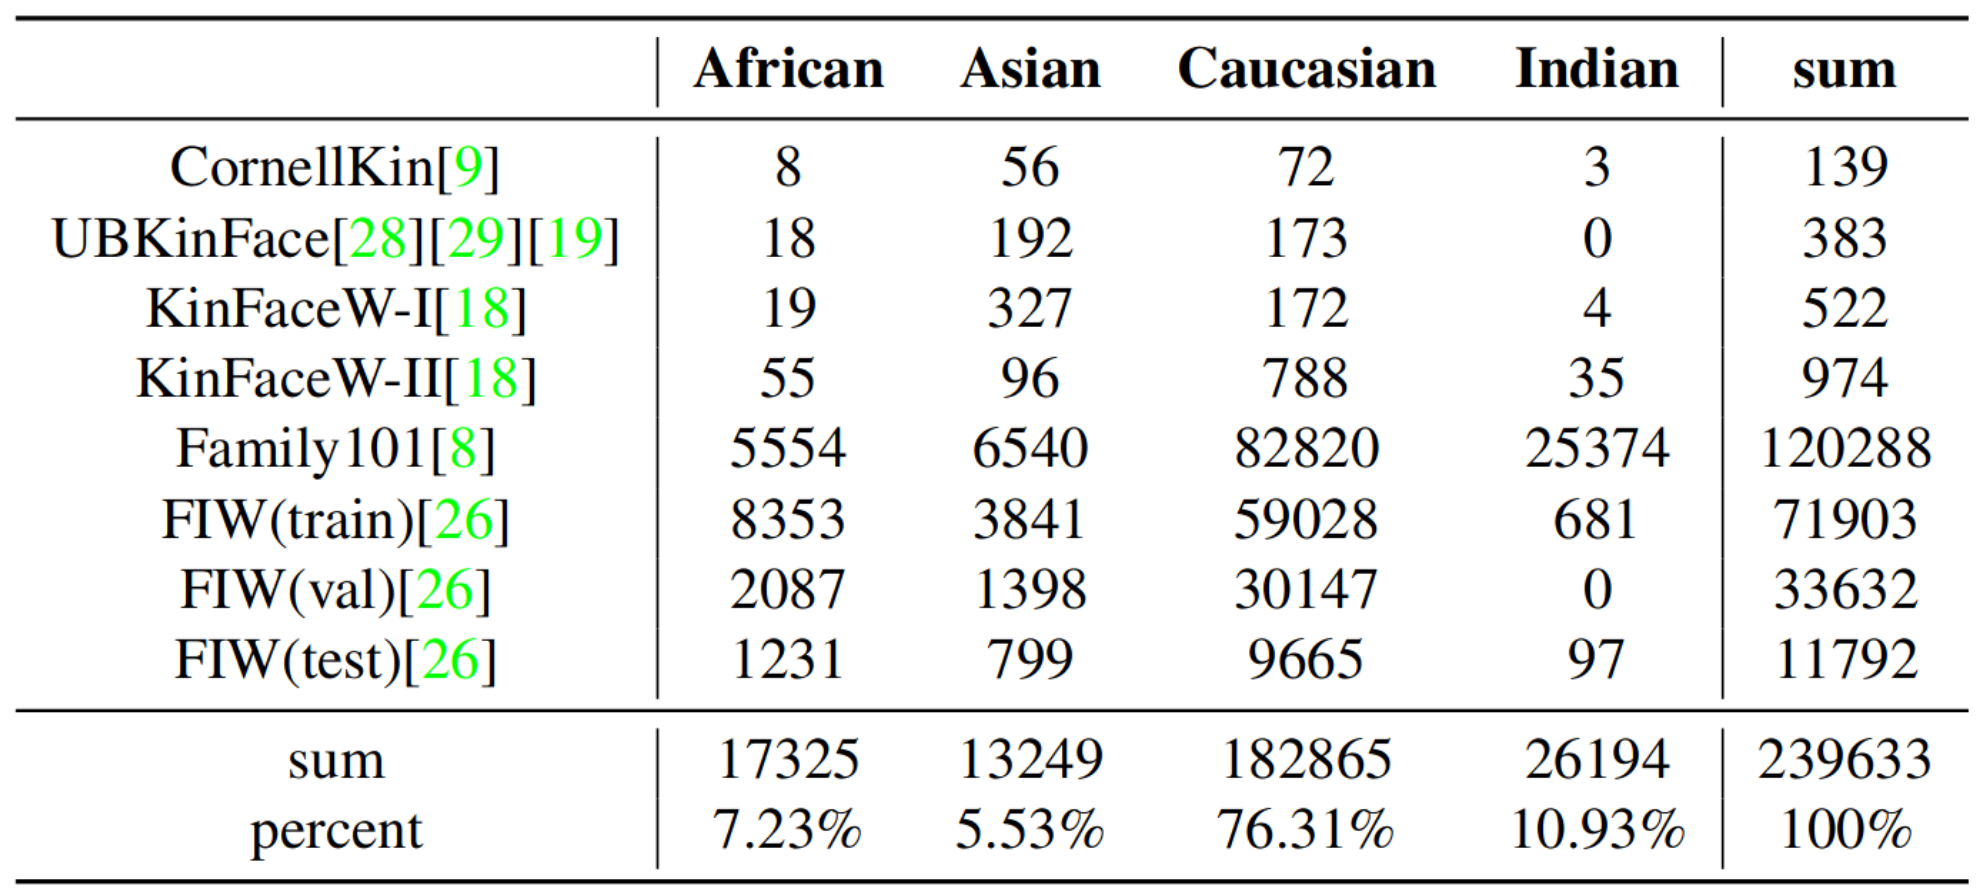
\includegraphics[width=0.75\textwidth]{imgs/2_Table1.png}
        \caption{From the authors. Dataset race distribution (approximately the same as the real-world distribution).}
        \label{fig:kfc-dataset-distribution}
    \end{figure}
    \begin{itemize}
        \item \textbf{Mixed-race} positive pairs are \textbf{removed}.
        %\item They manage to reduce race bias, but identity bias still exists, albeit limiting it to 30 images per person.  
        %\item Data quality alone doesn't significantly improve results, but being crucial to face verification, the authors plan to explore it in future works.
    \end{itemize}
\end{frame}

%------------------------------------------------
\section{Proposed Method}
%------------------------------------------------

\begin{frame}{Model Structure: overview}
    \begin{figure}
        \centering
        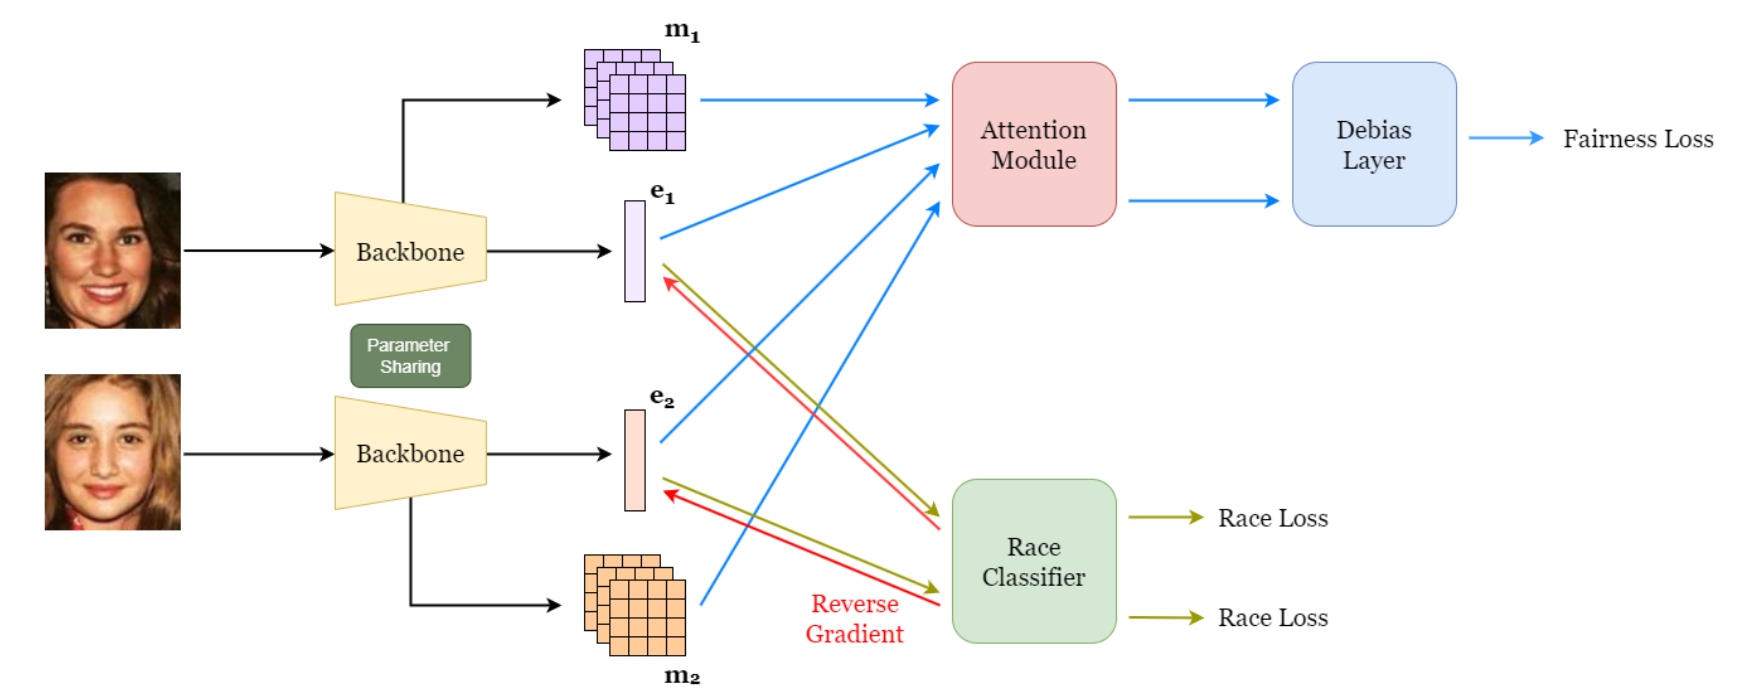
\includegraphics[width=0.75\textwidth]{imgs/3_KFC.png}
        \caption{From the authors. Overview of the proposed KFC model structure.}
        \label{fig:kfc-model-overview}
    \end{figure}
    %\begin{itemize}
    %    \item $e_1$ and $e_2$ are feature vectors from the backbone -- they are used for race prediction with gradient reversal.
    %    \item $m_1$ and $m_2$ are feature maps computed from backbone
    %    \begin{itemize}
    %        \item They are passed to attention module to extract import semantics and then passed to the debias layer to generate debias term in loss function.
    %    \end{itemize}
    %\end{itemize}
\end{frame}

%------------------------------------------------

\begin{frame}{Model Structure: attention module}
    \begin{figure}
        \centering
        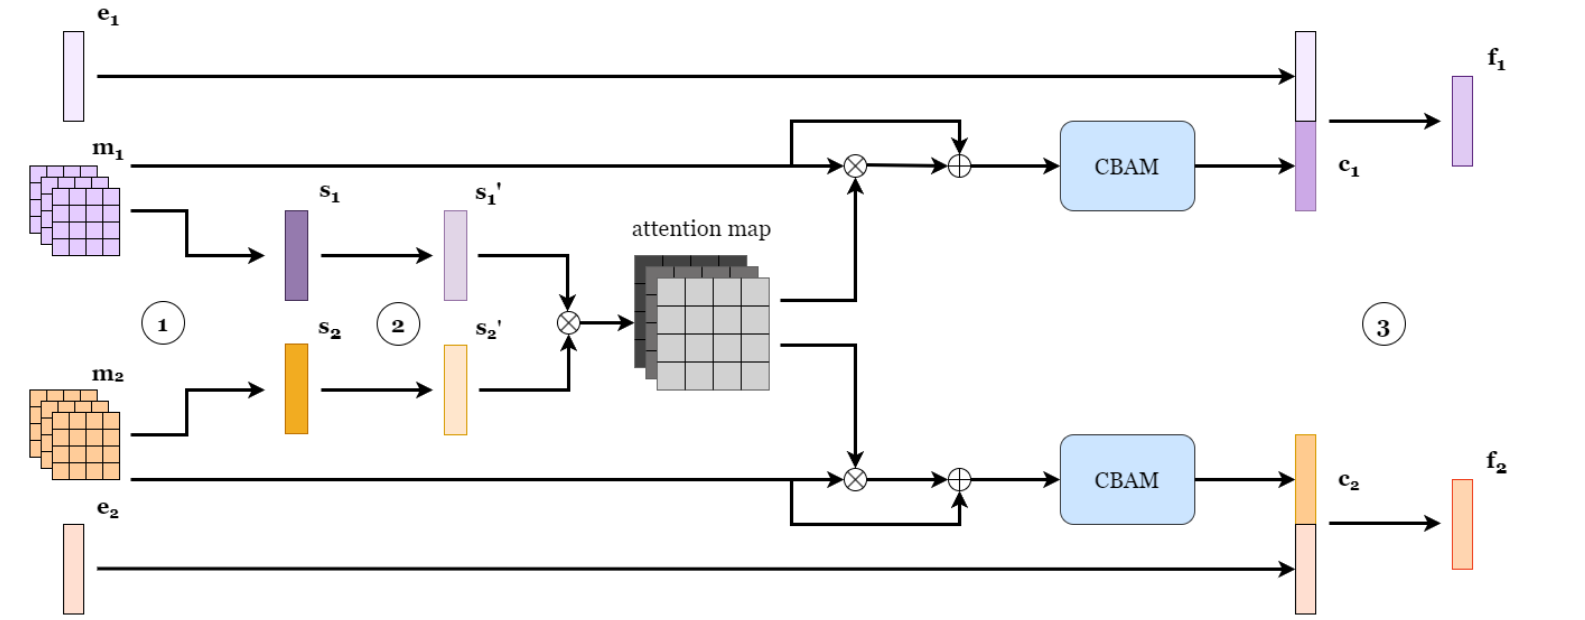
\includegraphics[width=0.75\textwidth]{imgs/4_AM.png}
        \caption{From the authors. Overview of the attention module. \circled{1}: average pooling, \circled{2}: 1x1 Conv with ReLU, \circled{3}: 2 layers of 1x1 Conv with ReLU.}
        \label{fig:kfc-attention-module}
    \end{figure}
    %\begin{itemize}
        %\item Inspired from R31, but with the average pooling for better accuracy and computational efficiency.
        % avg pool: interaction between different channels within a layer
        % added cbam: focus on the most relevant features to generate more sophisticated features.
    %\end{itemize}
\end{frame}

%------------------------------------------------

% \begin{frame}{Loss Function}
%     \begin{itemize}
%         \item The authors build on top of two previous works
%         \begin{itemize}
%             \item R46
%             \item R35
%         \end{itemize}
%     \end{itemize}
% \end{frame}
    
%------------------------------------------------

\begin{frame}{Loss Function: supervised contrastive loss}
    From \cite{R46}

    \begin{equation}
       L = \frac{1}{2n} \sum_{i=1}^{n} [L_c (x_i, y_i) + L_c (y_i, x_i)] \tag{1} 
    \end{equation}

    where

    \begin{equation}
        L_c (x_i, y_i) = - \log \frac{e^{s(x_i ,y_i) / \tau}}{\sum_{j=1}^{n} [e^{s(x_i ,x_j) / \tau} + e^{s(x_i ,y_j) / \tau}]} \tag{2}
    \end{equation}

    and $(x_i, y_i)$ is a \textbf{positive pair}, $(x_i, x_j)$ and $(x_i, y_j)_{j \neq i}$ are \textbf{negative pairs}, $s(x, y)$ is the \textbf{cosine similarity} between $x$ and $y$, and $\tau$ is a hyper-parameter used to control the degree of \textbf{punishment for hard samples}.
\end{frame}

%------------------------------------------------

\begin{frame}{Loss Function: MixFair Adapter}
    From \cite{R35}

    \begin{equation}
        \label{eq:mixfair-adapter}
        \cos(M(f_m), M(f_i))^2 - \cos(M(f_m), M(f_j))^2 = \epsilon \tag{3}
    \end{equation}

    where $(f_i, f_j)$ the identities' \textbf{feature maps}, $M(.)$ is the \textbf{debias layer}, and $f_m = \frac{1}{2} (f_i + f_j)$. If $\epsilon > 0$, then $i$ has larger \textbf{biases} than $j$, and vice versa.

    % mixfair - mixing the feature maps to remove bias
\end{frame}

%------------------------------------------------

\begin{frame}{Loss Function: fairness-aware contrastive loss function}
    \textbf{Combining} both previous works, they propose
    
    \begin{equation}
      L_{\text{fairness}} = -\log \frac{e^{\left(\cos(x_i,y_i) - b_i\right)/\tau}}{\sum_{j\neq i}^N \left[e^{\cos(x_i,x_j)/\tau} + e^{\cos(x_i,y_j)/\tau}\right] + e^{\left(\cos(x_i,y_i)-b_i\right)/\tau}} \tag{4}
    \end{equation}

    where $b_i$ is the averaging $\epsilon$ in Equation~\ref{eq:mixfair-adapter} representing the \textbf{bias between images} $I_i$ and other images in the same batch. Combining the temperature $\tau$ with the debias term $b_i$, they take into account both \textbf{accuracy and fairness}.
\end{frame}

%------------------------------------------------

\begin{frame}{Loss Function: race loss}
    In the \textbf{race classifier branch}, they use the \textbf{Cross-entropy} (CE) loss 

    \begin{equation}
        L_{\text{race}} = - \sum_{i=1}^n t_i \log(p_i) \tag{5}
    \end{equation}

    where $n$ is the total \textbf{number of races} in the training dataset, $t_i$ is the \textbf{ground truth} label, and $p_i$ is the \textbf{softmax probability} for the $i^{th}$ class.
\end{frame}

%------------------------------------------------

\begin{frame}{Loss Function: final loss}
    \textbf{Combining} the two previous loss functions, they have the \textbf{total loss function} given by

    \begin{equation}
        L_{\text{total}} = L_{\text{fairness}} + L_{\text{race}} \tag{6}
    \end{equation}
\end{frame}

%------------------------------------------------

\begin{frame}{Gradients of Fair Contrastive Loss Function}
    \cite{R34} analyzed the \textbf{gradients} with respect to positive samples $(x_i, x_i)$ and different negative samples $(x_i, x_j)_{(j \neq i)}$
    
    \begin{equation}
        \frac{\partial L(x_i)}{\partial \cos(x_i, x_i)} = -\frac{1}{\tau} \sum_{k \neq i} P_{i,k}, \quad \frac{\partial L(x_i)}{\partial \cos(x_i, x_j)} = \frac{1}{\tau} P_{i,j} 
    \end{equation}

    where $P_{i, j}$ is the \textbf{probability} of $x_i$ and $x_j$ being recognized as positive pair

    \begin{equation}
        P_{i,j} = \frac{e^{\left(cos(x_i, x_j)\right) / \tau}}{\sum_{k \neq i} e^{\left(cos(x_i, x_k)\right) / \tau} + e^{\left(cos(x_i, x_i) - b_i\right) / \tau}}
    \end{equation}

    \begin{block}{Summary}
    The authors validate the idea that a positive bias $b_i$ means a \textbf{stronger learning signal} ($P_{i,j}$ is larger) for positive and negative pairs. This fact implies a \textbf{faster training convergence}.
    \end{block}
    
\end{frame}

%------------------------------------------------

\begin{frame}{Fairness Mechanism}
    \begin{itemize}
        \item This work employs \textbf{two methods for improving fairness}: 
        \begin{itemize}
            \item Adversarial learning; and
            \item A fairness-aware loss function. 
        \end{itemize}
        \item The race classifier in adversarial learning \textbf{removes racial information} from feature vectors, which \textbf{decreases the performance standard deviation}. 
        %\item They note that adversarial training with a small dataset is not so effective. That's the reason they proposed the fairness-aware loss function.
        %\item Both methods decrease accuracy performance standard deviation across races while improving accuracy.
    \end{itemize}
\end{frame}

%------------------------------------------------
\section{Experiment}
%------------------------------------------------

\begin{frame}{Experimental Setting}
    \begin{itemize}
        \item Dataset
        \begin{itemize}
            \item \textbf{No overlapping families} between train, validation, and test sets;
            \item \textbf{Four races} (AA, A, C, I) -- ratios similar to Table~\ref{fig:kfc-dataset-distribution}; 
            \item \textbf{Four kinship relations} (FS, FD, MS, MD); 
            \item Images resized to \textbf{112x112} using MTCNN.
        \end{itemize}
        \item Implementation details (it follows \cite{R46})
        \begin{itemize}
            \item ArcFace model (backbone, \textbf{pre-trained} on ImageNet with ArcFace loss);
            \begin{itemize}
                \item Feature maps and feature vector of size $\mathbb{R}^{7\times7\times512}$ and $\mathbb{R}^{512}$, respectively.
            \end{itemize}
            \item Temperature $\tau = 0.08$ 
            %\item SGD with momentum = 0.9 and weight decay = 1e-4.
            \item SGD with \textbf{constant} learning rate* of $1e^-4$ and momentum of $0.9$.
            \item 10 epochs with 60000 steps; batch size = 25.
        \end{itemize}
        \item \textbf{Baseline} as the SOTA2021 \cite{R46}.
        \item In the following figures, \textbf{adversarial} means gradient reversal is enabled; for \textbf{multi-task}, there is not gradient reversal.
    \end{itemize}
\end{frame}

%------------------------------------------------

\begin{frame}{Ablation Study}
    \begin{figure}
        \centering
        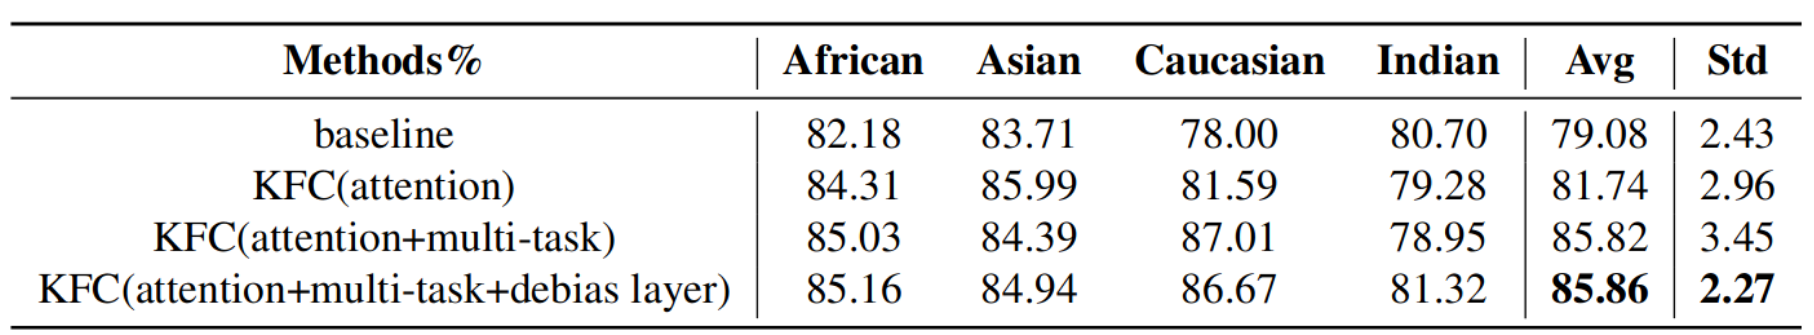
\includegraphics[width=0.75\textwidth]{imgs/5_Table2.png}
        \caption{From the authors. Ablation study on accuracy.}
        \label{fig:kfc-as1}
    \end{figure}
    \begin{block}{Effect of improving accuracy}
        With the attention mechanism, CBAM, and the race classification branch, the model learns features containing racial information, which adds a 7\% \textbf{improvement in accuracy over the baseline}. The debias layer also slightly \textbf{improves accuracy and standard deviation} by rectifying bias and making the compactness degree more uniform.
    \end{block}
\end{frame}

%------------------------------------------------

\begin{frame}{Ablation Study}
    \begin{figure}
        \centering
        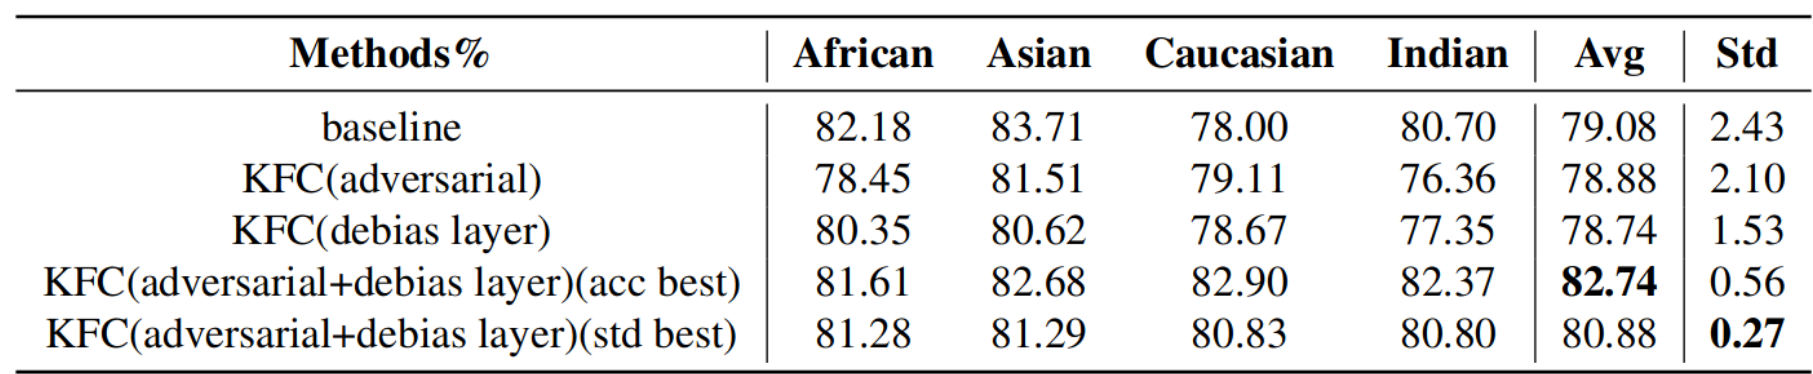
\includegraphics[width=0.75\textwidth]{imgs/6_Table3.png}
        \caption{From the authors. Ablation study on standard deviation.}
        \label{fig:kfc-as2}
    \end{figure}
    \begin{block}{Effect of improving fairness}
        Both fairness strategies (gradient reversal and debias layer) \textbf{mitigate bias} (reduce standard deviation), but also \textbf{harm accuracy}. By \textbf{merging} both strategies they remarkably \textbf{reduce standard deviation} while \textbf{boosting the accuracy}.
    \end{block}
\end{frame}

%------------------------------------------------

\begin{frame}{Comparisons with SOTA methods}
    \begin{figure}
        \centering
        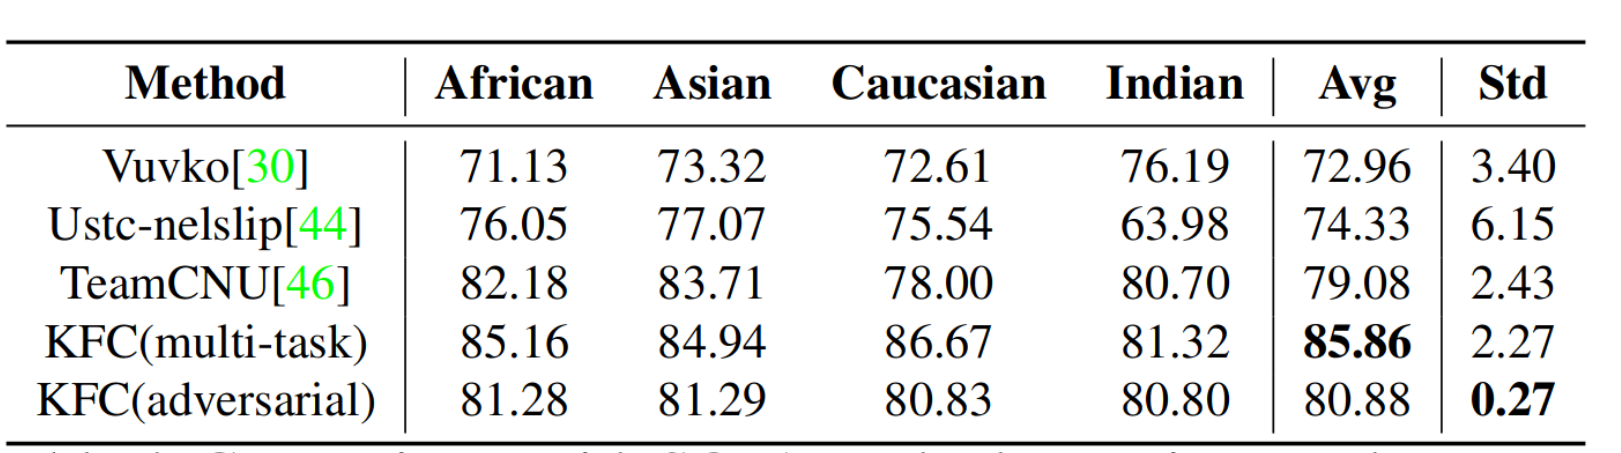
\includegraphics[width=0.75\textwidth]{imgs/7_Table4.png}
        \caption{From the authors. Comparisons with SOTA methods on KinRace dataset.}
        \label{fig:kfc-comparison-sota}
    \end{figure}
    \begin{itemize}
        \item These methods were \textbf{implemented} and \textbf{evaluated} on KinRace dataset.
    \end{itemize}
\end{frame}

%------------------------------------------------

\begin{frame}{Comparisons with SOTA methods}
\
    \begin{figure}
        \centering
        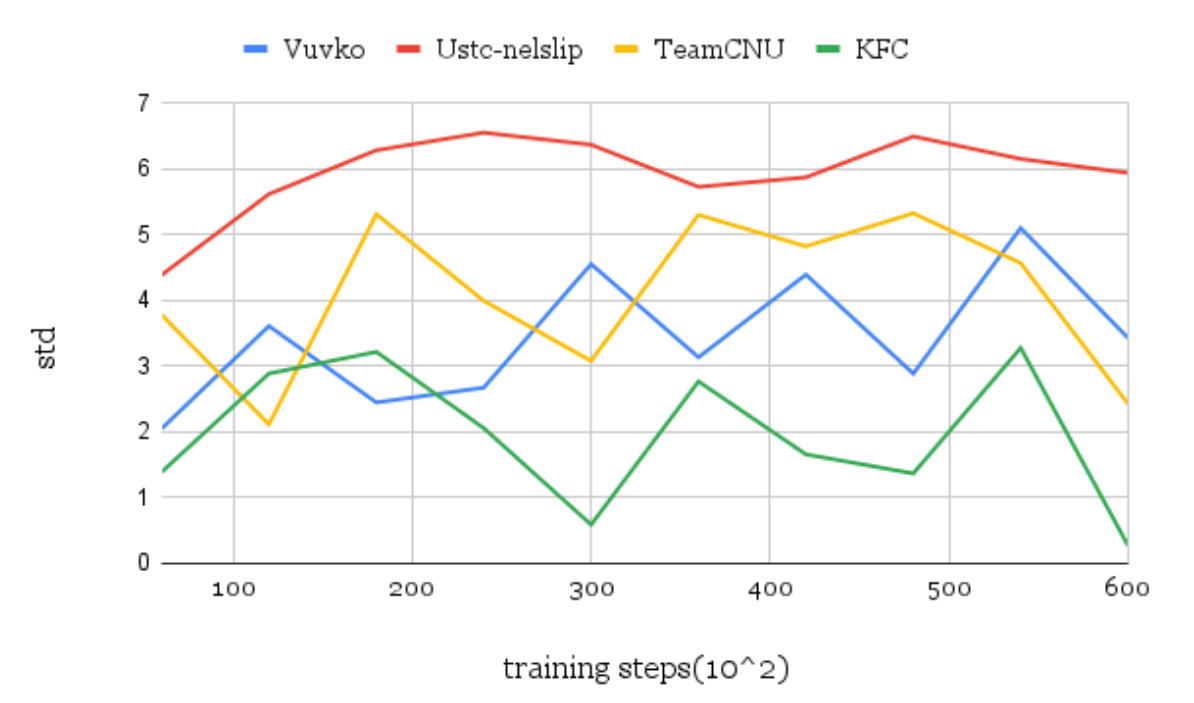
\includegraphics[width=0.5\textwidth]{imgs/8_Figure4.png}
        \caption{From the authors. Comparisons on standard deviation variations for different methods during training.}
        \label{fig:kfc-comparison-std}
    \end{figure}
    \begin{itemize}
        \item Standard deviation on the KinRace testing set every 10000 iterations on SOTA methods and the proposed KFC.
    \end{itemize}
\end{frame}

%------------------------------------------------

\begin{frame}{Comparisons with SOTA methods}
    \begin{figure}
        \centering
        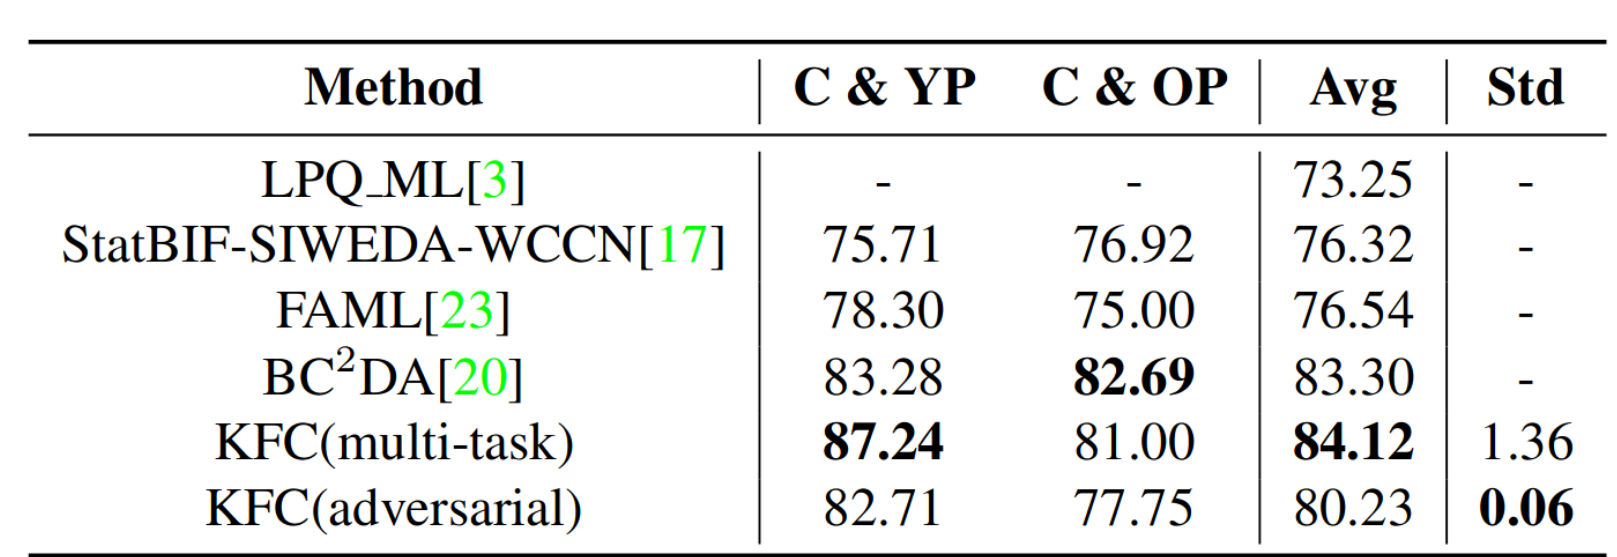
\includegraphics[width=0.75\textwidth]{imgs/9_Table5.png}
        \caption{From the authors. Comparisons with SOTA methods on UB KinFace dataset. This dataset provides child, young and old parent. C \& YP means child and young parent, and C \& OP means child and old parent.}
        \label{fig:kfc-comparison-ub}
    \end{figure}
    \begin{itemize}
        \item Multi-task version \textbf{outperforms} previous works, while the adversarial version \textbf{diminishes} the standard deviation significantly.
    \end{itemize}
\end{frame}

%------------------------------------------------

\begin{frame}{Comparisons with SOTA methods}
    \begin{figure}
        \centering
        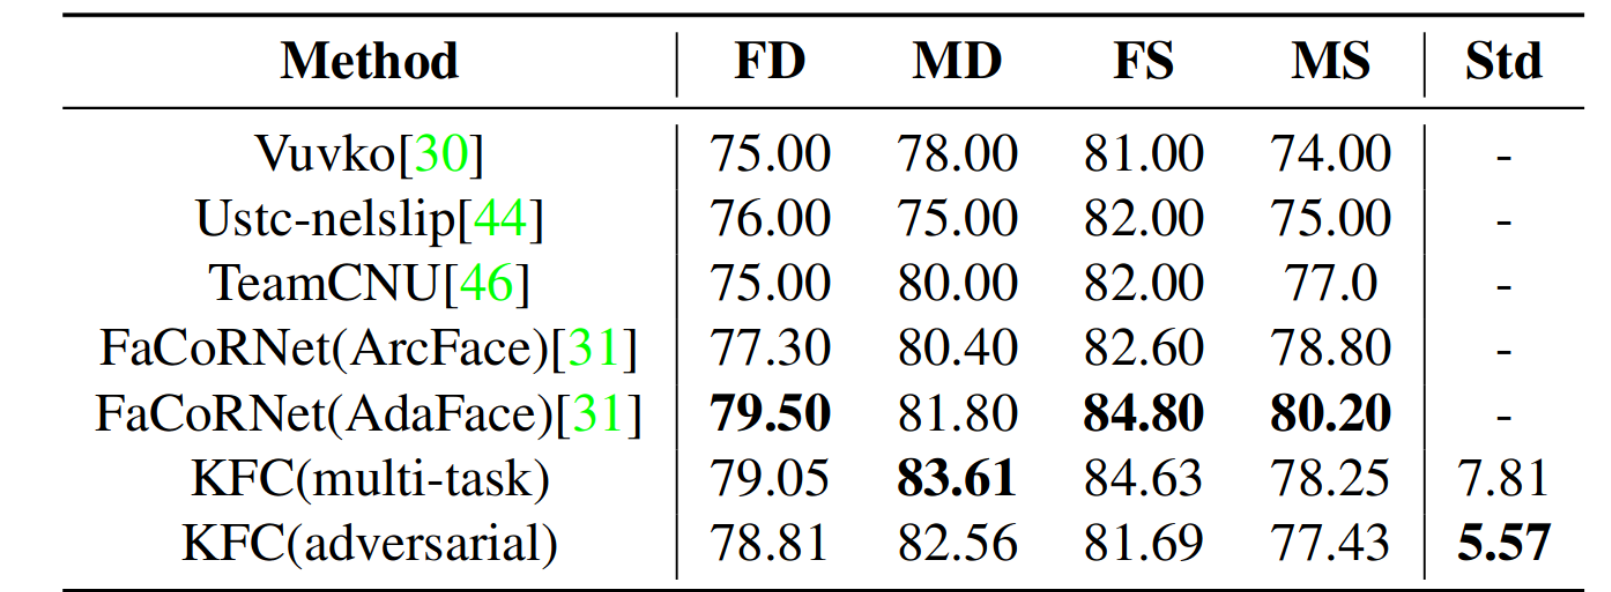
\includegraphics[width=0.75\textwidth]{imgs/10_Table6.png}
        \caption{From the authors. Comparisons with SOTA methods on FIW dataset.}
        \label{fig:kfc-comparison-fiw}
    \end{figure}
    \begin{itemize}
        \item The authors claim their results are \textbf{competitive} with \cite{R31}, but \textbf{better} because of their backbone (ArcFace vs. AdaFace).
        \item Additionally, their adversarial version \textbf{reduces} the standard deviation compared to the multi-task version.
    \end{itemize}
\end{frame}

%------------------------------------------------

\begin{frame}{Visualization and Analysis on Fairness}
    \begin{figure}
        \centering
        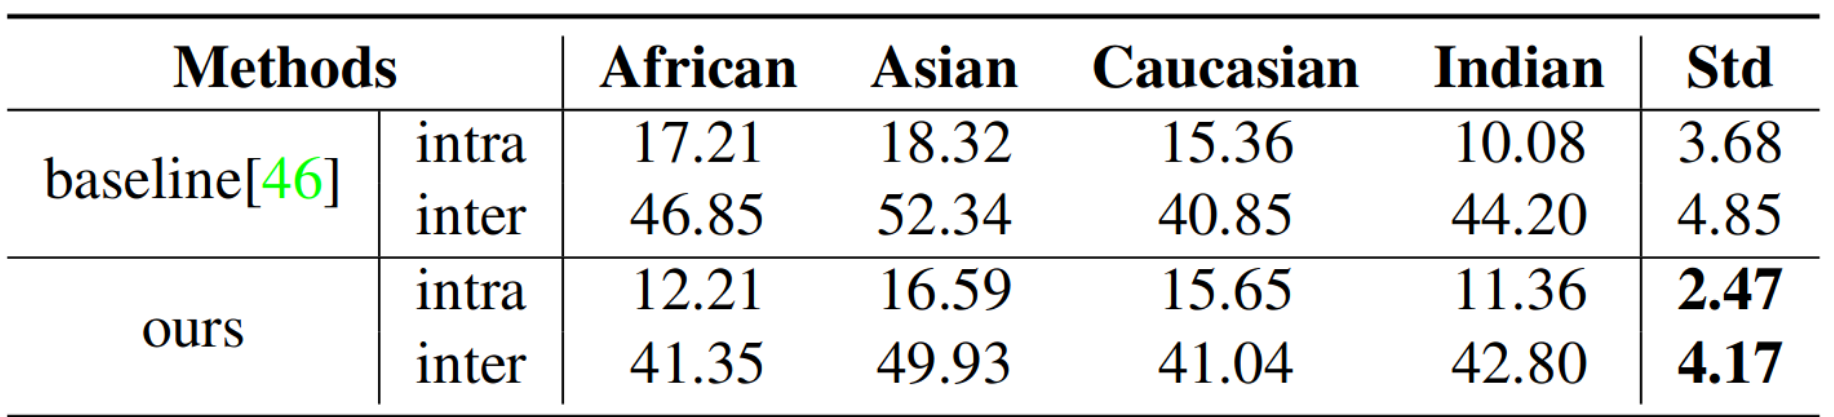
\includegraphics[width=0.75\textwidth]{imgs/11_Table7.png}
        \caption{From the authors. Intra-class and inter-class angle comparison. They randomly select 20 families per race from KinRace dataset.}
        \label{fig:kfc-comparison-angle}
    \end{figure}
    \begin{itemize}
        \item The KFC method \textbf{balances} the intra-class and inter-class angle between four races, which makes the compactness degree comparable, and thus markedly \textbf{improves fairness}.
    \end{itemize}
\end{frame}

%------------------------------------------------

\begin{frame}{Visualization and Analysis on Fairness}
    \begin{figure}
        \centering
        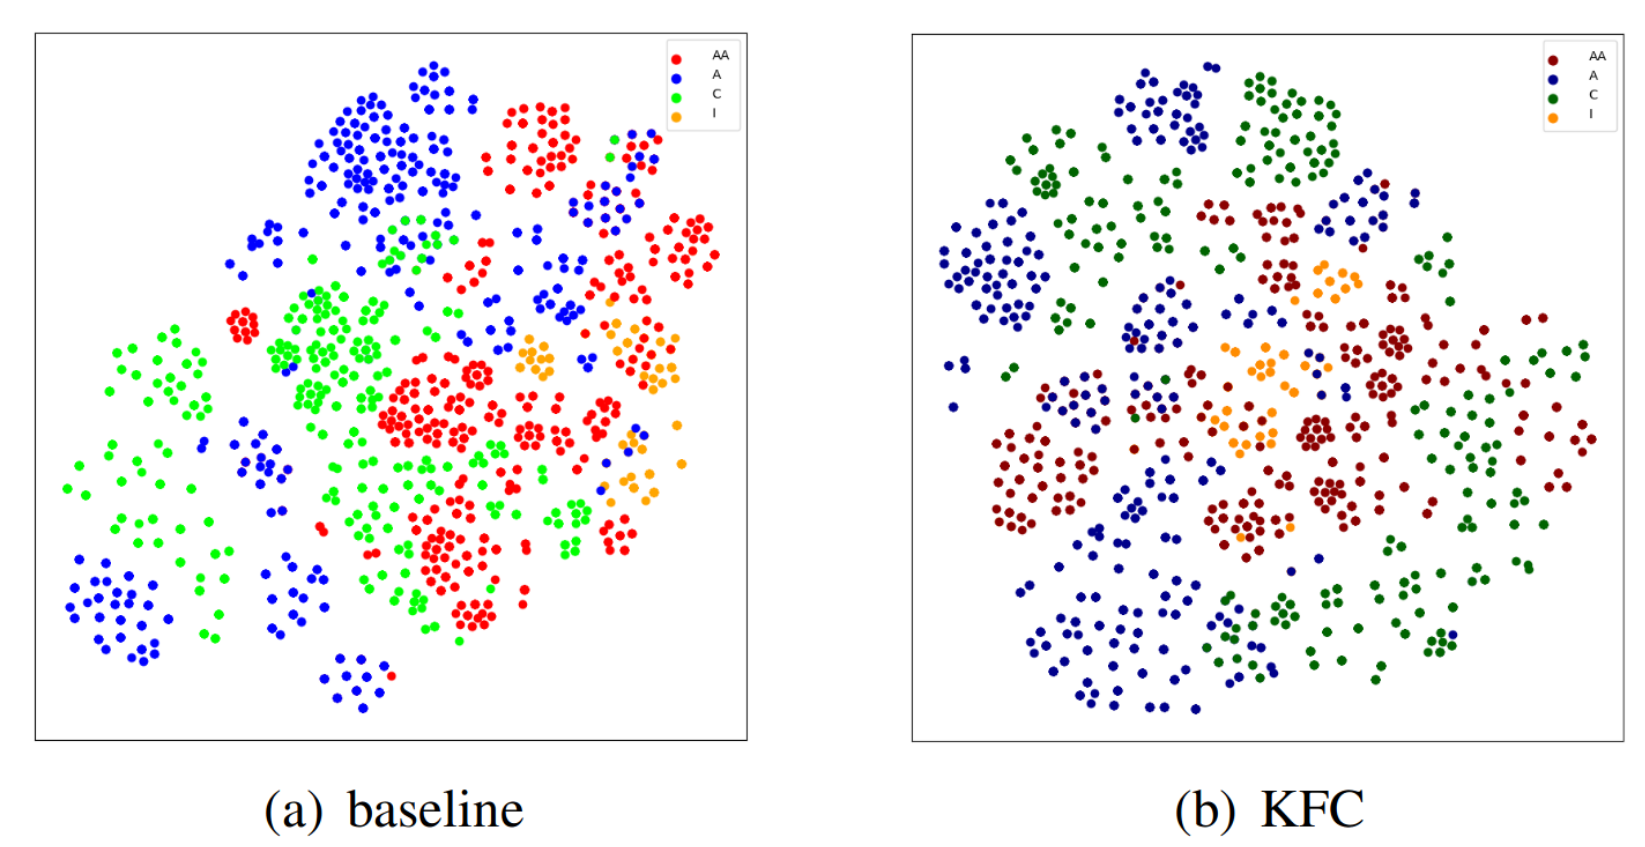
\includegraphics[width=0.5\textwidth]{imgs/12_Figure5.png}
        \caption{From the authors. t-SNE visualizations. They randomly pick 400 pairs per race from KinRace datset. AA for African, A for Asian, C for Caucasian, and I for Indian.}
        \label{fig:kfc-tsne-races}
    \end{figure}
    \begin{itemize}
        \item Feature embeddings are more \textbf{evenly distributed}; 
        \item \textbf{Clear boundaries} between the races were removed, which presents a \textbf{fairer solution} for kinship verification. 
        % \item To evenly distribute the embeddings means to remove clear boundaries between races. This implies that kinship verification has less race bias.
    \end{itemize}
\end{frame}


%------------------------------------------------
\section{Conclusion}
%------------------------------------------------
% TODO: also add my own conclusions
\begin{frame}{Conclusion}
    \begin{itemize}
        \item This work simultaneously aimed to \textbf{mitigate racial bias while improving accuracy} in kinship verification. 
        \item They used \textbf{adversarial learning} with a \textbf{fairness-aware loss function} in a \textbf{multi-task} model with an \textbf{attention} module. 
        \item A \textbf{kinship dataset} with racial labels, KinFace, was presented. 
        \item Their results suggest that their proposed method significantly \textbf{improves racial fairness} and \textbf{accuracy} for kinship verification by automatically adjusting intra- and inter-class angles in feature space.
    \end{itemize}
\end{frame}

%------------------------------------------------
\begin{frame}{References}
    % Beamer does not support BibTeX so references must be inserted manually as below
    \footnotesize{
        \begin{thebibliography}{99}
            \bibitem[Zhang, 2021]{R46} Zhang et al. (2021)
            \newblock Supervised Contrastive Learning for Facial Kinship Recognition
            \newblock 2021 16th IEEE International Conference on Automatic Face and Gesture Recognition (FG 2021)
            
            \bibitem[Shadrikov, 2020]{R30} Shadrikov, A. (2020)
            \newblock Achieving better kinship recognition through better baseline
            \newblock 2020 15th IEEE International Conference on Automatic Face and Gesture Recognition (FG 2020), pages 872–876
    
            \bibitem[Park, 2022]{R22} Park, S. et al. (2022)
            \newblock Fair contrastive learning for facial attribute classification
            \newblock In: Proceedings of the IEEE/CVF Conference on Computer Vision and Pattern Recognition. p. 10389-10398.

            \bibitem[Xu, 2021]{R42} Xu, X. et al. (2021)
            \newblock Consistent instance false positive improves fairness in face recognition
            \newblock In: Proceedings of the IEEE/CVF Conference on Computer Vision and Pattern Recognition. p. 578-586.
        \end{thebibliography}
    }
\end{frame}

\begin{frame}{References}
    % Beamer does not support BibTeX so references must be inserted manually as below
    \footnotesize{
        \begin{thebibliography}{99}
            \bibitem[Wang, 2022]{R39} Wang, Z. et al. (2022)
            \newblock Fairness-aware adversarial perturbation towards bias mitigation for deployed deep models
            \newblock In: Proceedings of the IEEE/CVF Conference on Computer Vision and Pattern Recognition. p. 10379-10388.
            
            \bibitem[Gong, 2021]{R11} Gong, S., Liu, X., Jain, A.K. (2021)
            \newblock Mitigating face recognition bias via group adaptive classifier
            \newblock In: Proceedings of the IEEE/CVF Conference on Computer Vision and Pattern Recognition. p. 3414-3424.
            
            \bibitem[Yu, 2020]{R44} Yu, J. et al. (2020)
            \newblock Deep fusion siamese network for automatic kinship verification
            \newblock In: 2020 15th IEEE International Conference on Automatic Face and Gesture Recognition (FG 2020). IEEE. p. 892-899.
            
            \bibitem[Su, 2023]{R31} Su, W. et al. (2023)
            \newblock Kinship Representation Learning with Face Componential Relation
            \newblock In: Proceedings of the IEEE/CVF International Conference on Computer Vision. p. 3105-3114.
        \end{thebibliography}
    }
\end{frame}

\begin{frame}{References}
    % Beamer does not support BibTeX so references must be inserted manually as below
    \footnotesize{
        \begin{thebibliography}{99}
            \bibitem[Raff, 2018]{R24} Raff, E., Sylvester, J. (2018)
            \newblock Gradient reversal against discrimination: A fair neural network learning approach
            \newblock In: 2018 IEEE 5th International Conference on Data Science and Advanced Analytics (DSAA). IEEE. p. 189-198.
            
            \bibitem[Gong, 2020]{R10} Gong, S., Liu, X., Jain, A.K. (2020)
            \newblock Jointly de-biasing face recognition and demographic attribute estimation
            \newblock In: Computer Vision–ECCV 2020: 16th European Conference, Glasgow, UK, August 23–28, 2020, Proceedings, Part XXIX 16. Springer International Publishing. p. 330-347.
            
            \bibitem[Wang, 2023]{R35} Wang, F.-E. et al. (2023)
            \newblock Mixfairface: Towards ultimate fairness via mixfair adapter in face recognition
            \newblock In: Proceedings of the AAAI Conference on Artificial Intelligence. p. 14531-14538.
            
            \bibitem[Wang, 2021]{R34} Wang, F., Liu, H. (2021)
            \newblock Understanding the behaviour of contrastive loss
            \newblock In: Proceedings of the IEEE/CVF Conference on Computer Vision and Pattern Recognition. p. 2495-2504.
        \end{thebibliography}
    }
\end{frame}

%------------------------------------------------

\begin{frame}
    \Huge{\centerline{\textbf{The End}}}
\end{frame}

%----------------------------------------------------------------------------------------
\end{document}